%
\documentclass[11pt,twoside,a4paper]{book}
\usepackage[shorthands=off,english]{babel} % package for multilingual support

\RequirePackage{iftex}
\ifPDFTeX
    \usepackage[utf8]{inputenc}
    \usepackage[T1]{fontenc}
    \usepackage{lmodern}
\else
    \RequirePackage{fontspec} % UFT8 fonts for LuaLaTeX
    \setmainfont{Latin Modern Roman}
\fi

\usepackage[ backend=biber
            , style=alphabetic
            , sortlocale=en_US
            , bibencoding=UTF8
            , maxcitenames=3
            , maxbibnames=100
            , giveninits=true
            ]{biblatex}

\usepackage{csquotes}
\usepackage{dirtytalk}
\usepackage{xcolor}
\definecolor{dark-red}{rgb}{0.6,0.15,0.15}
\definecolor{dark-green}{rgb}{0.15,0.4,0.15}
\definecolor{medium-blue}{rgb}{0,0,0.5}

\usepackage{minted}
\usepackage{pdfpages}
\usepackage{float}
\makeatletter
% custom float style, derived from ruled
% - caption is at the bottom
% - spaces before and after figure are larger
% - rules are thinner
\newcommand\floatc@botruled[2]{{\@fs@cfont #1} #2\par}
\newcommand\fs@botruled{\def\@fs@cfont{\bfseries}\let\@fs@capt\floatc@botruled
    \def\@fs@pre{\hrule\kern0.5\abovecaptionskip}%
    \def\@fs@post{\kern0.5\abovecaptionskip\hrule\kern0.5\abovecaptionskip}%
    \def\@fs@mid{\kern0.5\abovecaptionskip \kern0.5\abovecaptionskip}%
\let\@fs@iftopcapt\iffalse}
\makeatother
\floatstyle{botruled}
\restylefloat{figure}
\usepackage[labelfont=bf]{caption}

\addtolength{\textfloatsep}{-0.3cm}


\usepackage{graphicx}
\usepackage{xspace}
\usepackage{siunitx}
\usepackage{dsfont}
\usepackage{bytefield}
\usepackage{subcaption}

\newcommand\todo[1]{\noindent\textcolor{red}{(#1)}}

\newcommand{\FI}{Faculty of Informatics}
\newcommand{\MU}{Masaryk University}

\newcommand{\Jirik}{prof. RNDr. Jiří Barnat, Ph.D.}

\newcommand{\thesistitle}{Fault-tolerance for Metamorphic Robots}
\newcommand{\thesissubtitle}{PhD Thesis Proposal}
\newcommand{\thesisauthor}{Jan Mrázek}
\newcommand{\thesisYearCity}{Brno, 2020}
\newcommand{\thesisadvisor}{\Jirik}
\newcommand{\cpp}[1]{\mintinline[breaklines]{cpp}{#1}}

\addbibresource{bibliography.bib}

% widdow and club fix
\clubpenalty 10000
\widowpenalty 10000

\usepackage{setspace}
\usepackage{placeins}

\addtolength\textwidth{5pt}
\addtolength\oddsidemargin{1cm}
\addtolength\evensidemargin{-1cm}

\usepackage[inline]{enumitem}
\providecommand{\tightlist}{%
    \setlength{\itemsep}{0pt}%
    \setlength{\parskip}{0pt}%
    \setlength{\topsep}{0pt}%
    \setlength{\partopsep}{0pt}}

\usepackage[ pdfauthor={Jan Mrázek}
            , pdftitle={Fault-tolerance for Metamorphic Robots},
            , pdfsubject={PhD Thesis Proposal},
            , plainpages=false
            , pdfpagelabels
            , unicode
            , draft=false
            , colorlinks=true
            , linkcolor={dark-red}
            , citecolor={dark-green}
            , urlcolor={medium-blue}
            , unicode=true
            ]{hyperref}

% \punct command allows to shift the footnotemark above a punctuation
% Magic by František 'Fanda' Blahoudek
\newlength{\spc} % declare a variable to save spacing value
\newcommand{\punct}[1]{%
  \settowidth{\spc}{#1}% set value of \spc variable to the width of #1 argument
  \addtolength{\spc}{-1.8\spc}% subtract from \spc about two (1.8) of its values making its magnitude negative
  #1% print the optional argument
  \hspace*{\spc}% print an additional negative spacing stored in \spc after #1
}

\begin{document}

% \DocLength{evensidemargin}
% \DocLength{oddsidemargin}
% \layout

% initial pages from Mornfall + modifications

\frontmatter
\pagestyle{empty}

\begin{center}
    {\Large \sc \FI, \MU}
    \vskip4em
    \includegraphics[width = 4cm, height = 4cm] {logo_fi.pdf}
    \vskip4em
    {\begin{spacing}{1}
        \Huge \bf \thesistitle
    \end{spacing}}
    \vskip2em
    {\Large \sc \thesissubtitle}
    \vskip4em
    {\LARGE \bf \thesisauthor}
    \vfill
\end{center}
\textbf{Supervisor:}\\
\thesisadvisor \hfill \thesisYearCity

\cleardoublepage

% only in print version!
\iffalse %@ifprint

\section*{Statement of an author of a school work}

Student´s Name and UČO: Jan Mrázek, 422279

\vskip1em

I acknowledge that the Masaryk University (MU) is entitled in accordance with
the law (Article 35 § 3 and 4 of the Copyright Act No. 121/2000 Sb.) to use for
educational and other internal purposes on a non-commercial basis my thesis or
my other school work, which I authored to fulfill my study obligations towards
MU (my work).

The use of my work for internal purposes includes the use of the original work
as well as of its derivatives and might consists also of assigning of my work
for additional processing to another student or a member of the MU academic
community, or of making it available as a basis for a creation of a derivative
thesis or other school work at MU. Any such use of my work will acknowledge my
authorship, the original name and source of my work and will be conducted
exclusively in order to further develop educational and other interests of MU
related to further development and utilization of my work within its academic
community.

I also acknowledge my duty to inform MU at the latest upon the submission of my
work about my intent to further develop or use my work at MU or elsewhere or
about any other relevant issues related to my work.

\vskip2em

Brno, \today

\vskip2em

\hfill Student´s signature

\cleardoublepage

\fi

\section*{Declaration} % from Mornfall
Thereby I declare that this thesis is my original work, which I have
created on my own. All sources and literature used in writing the
thesis, as well as any quoted material, are properly cited, including
full reference to its source.

\vfill
\textbf{Advisor:} \thesisadvisor

\cleardoublepage

\section*{Abstract}

\todo{abstract}

\section*{Keywords}

\todo{keywords}

\cleardoublepage

\section*{Acknowledgements}

\todo{acknowledgement}

\cleardoublepage
\thispagestyle{empty}

\pagestyle{headings}
\pdfbookmark{\contentsname}{toc}
\tableofcontents
\mainmatter

\chapter{Introduction}\label{chap:introduciton}

Metamorphic self-reconfigurable robotics is one of the future challenges the
field of robotics is facing. The goal in this field is to design and develop an
autonomous robotic construction kit, which would allow for the construction of
sophisticated robots designed for specific tasks from smaller, simpler, and
unified autonomous units (modules). The advantage of such the approach lies in
its universality -- a single collection of modules can be reused multiple times
to fulfill a plethora of various tasks.

Moreover, the specific feature of metamorphic robots is that a bunch of
connected modules may autonomously change their mutual position and
interconnection to take a different physical shape, the ability referred to as
self-reconfiguration. As a result, various tasks may be completed within a
single mission by a single robot as it appropriately adapts its shape to fit the
individual mission requirements. Also, the self-reconfiguration property could
bring us closer to rapid prototyping of robots. We could treat robots just like
we treat software nowadays -- the developers just write robot description and by
\say{compiling} it, the robot self-assembles. Such ability would also allow for
version-control of robots with an easy option to roll-back to an older revision
without the necessity of keeping a physical inventory of older versions.

Metamorphic robots might also be a solution for building fault-tolerant robots.
A robotic system built out of large number of uniform modules could easily
recover from a module failure just like living organism survives the death of
individual cells.

Although the idea of metamorphic robots seems to be an appealing approach to
solve a variety of problems, the current state-of-the-art solutions are far from
practical applications. There are still too many unresolved problems ranging
from the theoretical to practical ones. These include, for example, the absence
of an efficient search for a reconfiguration plan, the lack of a unified
approach to modules' mass control, or the process of space miniaturization and
cost reduction \cite{4141032}.

\textcite{4141032} formulated challenges of the field of that time -- this
include hardware design, planning and control challenges. Most of the challenges
withstands to date. Few years later, \textcite{DBLP:journals/corr/abs-1108-5543}
propose the \emph{first grand challenge of modular robots}, after which
completion, we could consider advances in this field sufficient for practical
applications. They propose a scenario where 100 modules are placed in an unknown
area with walls and obstacles for 100 days. The modules are required to remain
active during the whole time without human intervention. The environment
provides power sources, however, they are not directly reachable by a single
module. Also, the location and the number of the power sources slowly change in
time so the robotic system has to adapt. To our knowledge, nobody was able to
finish the challenge so far. \todo{The closest to finishing the grand challenge
are} are the projects Symbricator \textcite{DBLP:conf/syscon/LeviMRKVSLC14} and
SMORES \textcite{DBLP:journals/arobots/JingTYK18}. Nevertheless, the research in
this field is vivid, and new results come every year.

While we can find results that deal with the theory of metamorphic robots and
works that deal with the physical implementation of metamorphic modules or
platforms, we see the advance in this field quite splattered and incoherent.
Research results that would interconnect both aspects of the problem appear
rarely. The situation is caused mainly by the fact that the physical design of
metamorphic modules is in many cases publicly unavailable, hence irreproducible.
As a result, researchers that are outside the original team of authors
practically cannot reuse the platform and build their research on top of the
previously known results.  Any reproducible and trustworthy research thus has to
be made either from scratch or based only on some guessed assumptions of what is
practical and realistic in case the researcher has no physical platform at hand.
Both cases significantly damper the research in the field.

In the rest of the thesis proposal, we first provide a general overview on the
area of metamorphic self-reconfigurable robots and present state-of-the-art in
the relevant subareas in Chapter \ref{chap:state-of-the-art}. Then we present
the selected challenges in the area of distributed and fault-tolerant control of
metamorphic robots I would like to tackle during my PhD study. We also give a
time schedule for my study in this chapter. In the Chapter \ref{chap:results} we
describe results we achieved so far and present \emph{RoFI} -- a new platform of
distributed metamorphic robots that is open-hardware and open-source, hence
almost freely available to anyone interested. Motivation behind this platform is
mainly to bridge the gap between theoretical and practical research in the
area.

\chapter{State of the Art}\label{chap:state-of-the-art}

A modular robotics is a way to build robots consisting of \emph{modules}. In
context of this paper, modules are rather high-level pieces with a certain level
of self-control instead of low-level components like individual actuators or
sensors. It might even make sense to talk about modules as individual robots,
which are used to build bigger robots. The modules have usually a limited set of
capabilities -- often the functionality is so primitive, the modules cannot
perform useful tasks on their own. However, when we join multiple modules, they
can cooperate and, therefore, new capabilities of the system as a whole emerge.
This idea probably first appeared in the work by
\textcite{DBLP:conf/icra/FukudaK90}, where they introduced CEBOTs (Cellular
Robotic System).

\section{Taxonomy of Existing Modular Robots}

Since the era of CEBOTs, many more projects followed and the research area split
into two: smart (or programmable) matter and modular robotics. The smart matter
aims at building very simple modules leveraging physical and chemical principles
(imagine artificial atoms) in order to create blob of modules, which can
reassemble into a different, usually solid, object based on an external input.
Contrary, the modular robotics aims at building more complex modules, which are
able of sophisticated self-organization (imagine artificial cells), which can
form usually highly dynamic robots that can autonomously move and interact with
their environment. Smart matter also aims at sub-millimeter modules, modular
robotics aims at sub-centimeter modules \cite{DBLP:conf/ieeealife/Christensen07,
1285597}. In the rest of this paper, we will omit smart matter and focus
exclusively on modular robots.

What distinguishes modular robots from swarm robotics is the ability of the
modules to mechanically connect and inherently form a larger robot. The
connection can be performed externally, e.g., by an operator, or the modules can
connect on their own. Even the trend is to build self-reconfigurable robots,
there are occasionally some exceptions, e.g., PetRo
\cite{DBLP:conf/ro-man/Salem14}.

There have been many more or less successful projects of self-reconfigurable
modular robots since the CEBOTs. The projects feature various designs approaches
from the capabilities of individual modules to the topology in which the modules
connect. Most of the projects used metamorphic modules, i.e., there is only a
single or a few types of modules in the system. We consider the following list
as a nice representable sample of the various designs: Fracta
\cite{DBLP:conf/icra/MurataKK94}, Molecule \cite{DBLP:conf/icra/KotayRVM98},
Polybot \cite{DBLP:conf/icra/YimDR00}, M-TRAN
\cite{DBLP:conf/icarcv/KurokawaKYTMK02}, Atron
\cite{DBLP:conf/iros/JorgensenOL04}, Superbot \cite{DBLP:conf/iros/SalemiMS06},
Molecube \cite{DBLP:journals/trob/ZykovMDL07}, Roombots
\cite{DBLP:conf/icra/SprowitzBDI09}, Symbricator
\cite{DBLP:journals/corr/abs-1109-2288}, SMORES \cite{DBLP:conf/iros/DaveyKY12},
M-Blocks \cite{DBLP:conf/iros/RomanishinGR13}, ModRED
\cite{DBLP:journals/ras/BacaHDND14}, HyMod \cite{DBLP:conf/dars/ParrottDG16} and
Omni-Pi-tent \cite{DBLP:conf/taros/PeckTT19}.

\textcite{4141032} distinguishes three categories of the robots based on the
topology in which they connect. Each category has its own specific problems of
control and makes some tasks easier than other:

\paragraph{Lattice architecture} have its modules arranged in regular 3D grid --
e.g., a cube or hexagonal grid. The modules are tightly packed together. Typical
examples of such architectures are M-Blocks \cite{DBLP:conf/iros/RomanishinGR13}
and Atron \cite{DBLP:conf/iros/JorgensenOL04}. The regular grid makes it easier
to create a reconfiguration schedule and execute in parallel (for more details
see Subsection \todo{ref}). However, reconfiguration is usually the only option
for locomotion of such system, and, therefore, lattice architectures do not
yield highly dynamic systems.

\paragraph{Chain architecture} have its modules connected in a string or
possibly in a tree. Typical examples of such architectures are Polybot
\cite{DBLP:conf/icra/YimDR00} and Molecubes
\cite{DBLP:journals/trob/ZykovMDL07}. This architecture allows for easy
formation of limbs and arms, therefore, these robots usually interact well with
the environment. Also even very simple controllers yield locomotion (via
snake-like movements (see Subsection \todo{ref} for more details). The chains
can also form space-filling curve, therefore, e.g., Molecubes, can form a
lattice-like structures, while the underlying structure is linear.

\paragraph{Hybrid architecture} allows for both arrangements of modules,
therefore combines the advantages of both, possibly at the cost of increased
complexity. Examples of such robots are M-TRAN~III
\cite{DBLP:journals/ijrr/KurokawaTKKHM08}, Roombots
\cite{DBLP:conf/icra/SprowitzBDI09}, SMORES \cite{DBLP:conf/iros/DaveyKY12},
HyMod \cite{DBLP:conf/dars/ParrottDG16} and Omni-Pi-tent
\cite{DBLP:conf/taros/PeckTT19}. We can perceive that the most recent trend is
to build hybrid architectures. Especially SMORES are designed to be able to
replicate arrangements of the other platforms, thus be as versatile as possible
\cite{DBLP:conf/iros/DaveyKY12}.

On top of the locomotion provided by the the inter-module interaction, some
systems feature locomotion of the individual modules - e.g, by providing wheels
(SMORES, HyMod) or tracks (Symbricator), which further makes the reconfiguration
problem easier by allowing the modules to move on their own in the space without
interaction with the rest of the modules. A good example of such solution is
work by \textcite{DBLP:journals/ral/LiuWY19}.

\section{Challenges of Modular Robots}

There are many common challenges of modular robotics and the robotics in
general. This challenges were nicely summarized recently in blog post by
\textcite{locklin_2020}. Most of the challenges can be characterized by shifting
the robots from single purpose devices used in industrial automation, which
follow a preprogrammed path ignoring any environment around them, to autonomous
devices which can move in and interact with environment and adapt to its
changes. The challenges includes problems like motion planning (how to get from
point A to point B and avoid obstacles), continuous mapping of the environment,
scene understanding, and affordance discovery (predicting how the object will
behave when the robot interacts with it).

In the rest of this paper, we will focus only on the challenges specific to
metamorphic robots. We will also deliberately omit the challenges of mechanical
and electrical design of such robots. We will only slightly touch them in
Section \ref{sec:mixed-challenges}.

Let us introduce the challenges and illustrate them on a simple case. Suppose
there is a robot composed out of the modules in a simple environment. See figure
\ref{fig:arena} for illustration of the environment. There are two elevated
ramps. On one of them, there is red cube. The robot is supposed to move the cube
from one ramp to another. There is also a power socket after a narrow passage.
The modules do not have enough energy to complete the whole task.

\begin{figure}[!t]
    \centering
    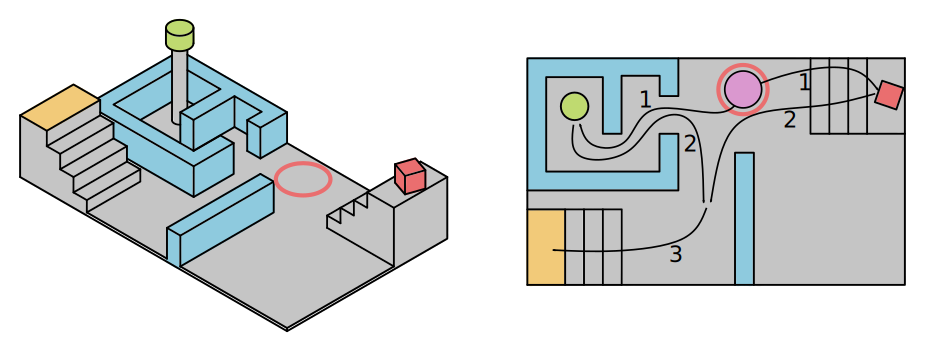
\includegraphics[width=0.7\textwidth]{figures/arena.jpg}
    \caption{The example environment for illustration of various challenges of
    self-reconfigurable robots.}
    \label{fig:arena}
\end{figure}

Once the robot is given the task, \footnote{Note, that for our purposes we omit
the translation step from "move the cube" to having a precise program saying
move to point A, grab a cube, move to point B, release the cube. We omit it as
we consider the translation as an open general problem of robotics.} we expect
it to find a plan to fullfil the task.

One of the possible solution is to first split in half and form two robots --
one will go to harvest energy, the second one will go and grab the cube. Then
then will join again on the way to the second ramp and share power. To do so,
the energy harvesting robot reconfigures into and energy efficient configuration
for locomotion and moves toward the narrow passage. Before the passage, it
reconfigure itself into a snake and passes it. Then it forms an arm and reaches
the power socket to charge itself. Meanwhile, the other robot moves towards the
first ramp. When it reaches the ramp, it changes shape so it can crawl the ramp
ramp and to grab the red cube cube. Then it returns and reunions with the energy
harvesting robot. They form a single robot and share the harvested power. During
climbing the other ramp, one of the modules in the systems stops responding,
therefore, however, the robot still continues to operate -- it just moves
slower. Before reaching the top of the ramp, the robots falls. It survives by
breaking inter-module connections to prevent module damage. The robots
reassembles and finishes the task.

Other possible solution (more suitable for cell-like robots, e.g., ATRON) is to
move in a \say{liquid blob of mass} which surrounds the cube and nudges it in
the desired direction.

In this simple example, we can identify several challenges typical for
self-reconfigurable robots. The first, obvious one, is \emph{planning
challenge}. The robot has to analyze the problem and figure out how to leverage
its ability to change shape to fulfill the task. The second challenge is the
challenge of \emph{locomotion} of the whole group of robots. Even the individual
modules can have wheels to move themselves, it is desirable to move in blocks as
new locomotion capabilities will emerge -- e.g. individual modules are not able
to climb stairs, but a system of them is. The next challenge is the
\emph{reconfiguration challenge}. This one is straightforward -- the robots have
to have an algorithm to compute reconfiguration plan to change shape. To
actually locomote, compute and schedule the reconfiguration we are facing the
\emph{control challenge}. We have to be able to control large number of modules
in a synchronized manner and ideally leverage all their computational potential.
All of the above should be designed in fault-tolerant way otherwise the large,
complex system will certainly fail. Also, the system has backed by solid
hardware and software solutions, which presents the \emph{mixed hardware and
software challenge}.

In the following section, we will discuss state-of-the-art for each of the
challenges individually.

\section{Planning Challenge}

For the purposes of this thesis, we consider planning for modular robots as an
effort to leverage the shape-changing ability of the self-reconfigurable robots
to fulfill tasks as efficient as possible and to adapt to an unknown or changing
environment. Note that planning often denotes also reconfiguration or locomotion
in the literature. For brevity, we also exclude work dealing with planning for a
single robot.

Despite we presented number of projects, nearly none of them deals with
planning. Instead, they focus rather on low-level control (locomotion and
reconfiguration), which we will cover in the later sections. To our knowledge,
there are two research groups that presented results in the area of high-level
planning of self-reconfigurable robots: SMORES and Symbricator.

There are several publications dealing with high-level planning for SMORES.
\textcite{DBLP:journals/arobots/JingTYK18} present a automata-based planner
(extension of their previous work \cite{DBLP:conf/ijcai/JingTYK17}), which takes
a task objective written in a \emph{Structured English}
\cite{DBLP:conf/iros/FinucaneJK10}. Their planner leverages a library of
handcrafted configurations. Each configuration have a set of properties and a
set of associated low-level controllers, which can perform single high-level
task -- e.g., move forward. The planner simply switches between those
configurations and controllers to achieve the specified goal. The switching is
based on a finite automaton. The automaton is synthesized from a set of formulas
in linear temporal logic (LTL) using an approach presented in
\cite{DBLP:journals/trob/Kress-GazitFP09}. The formulas come from the task
objective and additional constraints of the individual library configurations.
Note, that this approach is not brand new -- it was already introduced in
\cite{DBLP:conf/iros/CastroKK11} for CKBots, but work by
\textcite{DBLP:journals/arobots/JingTYK18} we just discussed, makes the approach
more robust and they present much more challenging experiments.

There is also work by \textcite{DBLP:conf/icra/TosunDJKCY18} on planning for
SMORES. They use a similar approach leveraging a library of hand-crafted
configuration as \cite{DBLP:journals/arobots/JingTYK18}. However, they extend
the system with \emph{environment augmentation modules} (just like
\cite{DBLP:conf/rss/PetersenNW11}) -- basically a passive modules serving as
building blocks for bridges and ramps, that can be used to augment the
environment, hence making fulfilling the objective easier for the robots.

Both of the presented approaches for SMORES use an external environment feedback
in the form of cameras with environment objects being tagged by black and white
patterns \cite{DBLP:journals/scirobotics/JingTYKC18}.

\textcite{DBLP:conf/syscon/LeviMRKVSLC14} take a different point of view on
planning for Symbricator. They focus and discuss mainly long-term plans for a
robotic system. Therefore, they propose that the planners should first focus on
the survival of the systems first (e.g., charging itself), and then, when
survival is guaranteed, the system should perform given tasks. Their
contribution lies in introduction of the \emph{SOS cycle}
(swarm-organism-swarm). In the cycle, the modules should first discover the
environment on their own (e.g., map it and locate power sources), then they
share the gathered information about environment. Then the modules assemble
together and fullfil a task. Once the task is completed (or failed), the modules
disassemble and the cycle repeats. In \cite{DBLP:conf/syscon/LeviMRKVSLC14},
they present advances on individual phases of the cycle (locomotion,
self-assembly, environment mapping). They also introduced concept of global
motion planning in \cite{DBLP:conf/icra/VonasekSKP13} using RRT
(rapidly-exploring random tree). This is an extension of the previous work
\cite{DBLP:conf/taros/VonasekKP12} by motion primitives -- a controllers for
specific configurations just like in the case of high-level planning for SMORES
\cite{DBLP:journals/arobots/JingTYK18}.

\section{Challenge of Reconfiguration}

There is a variety of work dealing with the reconfiguration problem. The work
differs by problem specification, used approaches and a mathematical model of a
robotic system.

Most of the work considers reconfiguration from given initial configuration to
given target configuration on chain or hybrid module types. The expected output
of the reconfiguration is a sequence of connect/disconnect operations and joints
movements to perform in order to reach the target configuration. Since all the
movements take time to complete and consume energy, it is desirable to find the
shortest reconfiguration sequence. Also, it is highly beneficial if the
reconfiguration plan can be computed in distributed manner to leverage the
computation power of the individual modules.

Exploration of the state-space of the system is a straightforward approach.
However, as \textcite{DBLP:journals/jfr/ChirikjianPE96} showed, the number of
possible configurations grows exponentially, therefore, direct explorations is
infeasible even for small systems. \textcite{DBLP:conf/iros/AsadpourASI09}
showed edit distance heuristics, that can improve performace of the search and,
therefore, increase size of the configuration which is manageable by this
approach. \textcite{DBLP:conf/monterey/BaarirHKR10} tackle the problem of large
state-spaces by using a symbolic representations inspired from software model
checking. All the work above demonstrates the results on MTRAN-like modules.

Since the modules in a system are from the reconfiguration point of view
indistinguishable from each other, we should treat isomorphic configuration as
the same. There are some advances in this area leveraging specific properties of
the robotic systems presented in \textcite{DBLP:journals/ijrr/ParkCTY08},
\textcite{DBLP:conf/iros/AsadpourASI09} and
\textcite{DBLP:journals/ras/TaheriMAP16}.

One of the most interesting results in reconfiguration is done by
\textcite{DBLP:journals/ras/HouS14}. They introduce a model of robotic system
called a \emph{connector graph}). They show that the problem of finding the
shortest reconfiguration plan between two connector graphs is NP-complete. They
provide an exponential distributed algorithm and also an approximative
distributed algorithm running in polynomial time for the problem. Since
connector graphs capture only topology, this approach produces only
connect/disconnect actions. Hence, it might produce a plan which is not
collision-free and cannot be executed due to physical limitations. Such plans
are suitable for robots with good self locomotion (e.g., SMORES) but hard-to-use
in a system lacking individual modules locomotion (e.g., M-BLOCKS or M-TRAN).
When the modules can move on their own, they can simply disconnect from the
system, move to the target location, and connect there as presented in
\cite{DBLP:journals/ral/LiuWY19}.

As the reconfiguration on connector graphs is NP-complete,
\textcite{DBLP:journals/pcs/GorbenkoP12} present a solution to the
reconfiguration via reduction to the Boolean satisfiability problem (SAT).

Other results aim at finding a feasible plan rather than the shortest one. To
name a few, \textcite{10.1117/12.360345} use the divide and conquer approach.
\textcite{DBLP:conf/icra/HouS08} present a reconfiguration emerging from local
behaviors in tree configurations. \textcite{DBLP:journals/ral/LiuWY19} use
dynamic programming for reconfiguration between tree configurations.

\textcite{DBLP:conf/iros/ButlerBR01} present a \emph{Pac Man} algorithm for
transportation of modules on the 2D perimeter of a lattice robot with cube
modules. This algorithm is a base for naive reconfiguration -- by simply sending
one module by one to the goal destination. The Pac Man algorithm was extended to
3D surface a year later in \cite{DBLP:conf/wafr/ButlerR02}.
\textcite{DBLP:journals/dc/WalterWA00} gives a distributed algorithm, which is
however incomplete -- there exists configurations between it is not able to find
reconfiguration path. \textcite{DBLP:conf/icra/VassilvitskiiYS02} present a
distributed algorithm for reconfiguration of lattice type robots, which is
complete with only one restriction: they use $2\times2\times2$ meta-modules for
the reconfiguration. The initial and target configurations have to overlap at
least on one meta-module. \textcite{DBLP:conf/ieeealife/Christensen07} adapt
similar approaches for ATRONs. They use meta-module composed out of three
modules. They compute reachable positions on the surface of a blob of modules
and then move the meta-module along the shortest path on the surface. They can
also move multiple modules in parallel. Later,
\textcite{DBLP:journals/comgeo/AloupisBDDFIW13} presented asymptotically better
algorithms for reconfiguration of lattice type robots using non-uniform
meta-modules.

The results above were not demonstrated on large scale in practice. Contrary to
that, \textcite{DBLP:conf/iros/RomanishinMR19} present an online distributed
algorithm for M-BLOCKS to reconfigure into a line, which they were able to
demonstrate on physical robots in various conditions. Quite recently,
\textcite{DBLP:journals/ras/HauserMLKBI20} presented and experiment, where 12
Roombot modules reconfigure into a chair. The algorithm used for reconfiguration
takes in account the limited strength of the joints.

The approaches presented above yield deterministic reconfiguration plan.
\textcite{4141032} appeled that stochastic reconfiguration approaches should be
applied to modular self-reconfigurable robots. To our knowledge, to date
stochastic reconfiguration is widely used for smart-mattery and similar
minimalistic modular robots (e.g., Catoms \cite{DBLP:conf/aaai/KirbyCAPHMG05})
but have not been widely adapted for \say{full-featured} modular robots we are
interested in in this paper.

% There are also approaches considering module position in space during the
% reconfiguration. These are usually motivated by the locomotion of the whole
% system of modular robots: \textcite{DBLP:conf/robotik/BonardiMSVI12} present some
% locomotion primitives for Roombots, \textcite{mtranMotion} present an algorithm for
% locomotion through reconfiguration of M-TRANs. \textcite{M-block-line} present a
% reconfiguration to a line using M-BLOCKS considering the position of the modules
% in space. Another approach is used by \textcite{Femtobots} -- they pre-synthesize
% individual module locomotion on the surface of a given scaffold and then
% consider to build larger configuration containing only these scaffolds.


\section{Challenge of Locomotion}

\todo{Not sure if this will be covered by control and planning or not}
\todo{Present the special kinematics}

\todo{Self-Reconfigurable Modular Robots – Hardware and Software Development in AIST - lattice is not good at movement}

\section{Control Challenge}

\todo{ Somewhere show the relation to inverse kinematics and the new SMORES paper}

\todo{Explain, why central control is bad}

\todo{Show, how the robots can communicate and why sometimes it is bad.}

\todo{Explain difference between reconfiguration and locomotion, say you will show examples later}

\todo{Explain, common approches to controlling the robots in a distributed
    manner. Present case studies and experiments in the following points:}

\todo{Present gait tables and basic synchronization approaches for them }

\todo{Present digital hormones}

\todo{Present nested controllers}

\todo{Also present the central solutions tackling the grand challenges - e.g. the SMORES navigation paper }


\section{Fault-tolerance Challenge}

There is no single widely accepted interpretation of what fault tolerant systems
should comply to. Usually, in a context of embedded system, a system is
considered fault-tolerant when it is able to continue operating (possibly with
worse performance) after one of its components fails
\cite{DBLP:journals/micro/Johnson84}. The extent of fault-tolerance depends on
what type of failures the system survives.

For example, we usually consider living organisms as highly fault-tolerant
systems. If an animal looses an limb, it is able to adapt and perform similar
tasks. E.g., a cat without a leg is still able to move and climb -- possibly
slower, but it is able to survive.

In the context of metamorphic robots, \textcite{DKbotDistr} discuss several
aspects of fault-tolerance and for some of them they propose solutions. They
distinguish several types of fault:

\paragraph{Complete module malfunction,} where the module stops responding and
acts passively. The usual assumption is that the other modules in the system can
detect such module. This type of malfunction is probably the most mentioned one
in the literature. The usual solution is to either drop or to ignore such
modules and reconfigure into a new configuration
\cite{DBLP:conf/ieeealife/Christensen07, DMotionCoord}.

\paragraph{Byzantine module malfunction,} where it is not easy to detect the
module has failed -- e.g., the module can have a wrong sensor and it can report
wrong data to other modules. The module can even be malicious. There is not much
work on this type of malfunction in the context of metamorphic robots as far as
we are aware. However, in context of distributed systems in general, it is a
vivid research topic. E.g., work by \textcite{DBLP:conf/osdi/CastroL99} could be
adapted for metamorphic robots.

\paragraph{Actuator malfunction,} where the module control unit is fully
functional, however, one or more of the modules actuators are either stuck
in a position or spin freely. This type of malfunction was tackled by
\textcite{DBLP:conf/romoco/VonasekONW15}.

\paragraph{Explosion of the whole system} is a type of malfunction where the
robot is broken down into pieces randomly spattered over the environment usually
after a high energy impact. \textcite{DBLP:conf/iros/YimSSPDT07a} proposed a
solution for automatic reassembly after explosion. They also discuss, that
system explosion is a way of fault-avoidance. When a system can reassemble, it
is desirable to include weak, re-attachable joints, which protect the individual
modules.

\todo{This section misses more in-depth references for existing solutions}

\section{Mixed Software and Hardware Challenges}\label{sec:mixed-challenges}

\todo{Docking!}
\todo{Raise question about hardware reliability}
\todo{Raise question about firmware distribution}
\todo{Raise question about security of such robots}
\todo{Point that we can solve all above individually, but we lack a single platform offering all of them and we also suck at miniaturization a making cheap modules}


\section{Availability of various Robotic kits}
% The system can be \emph{centrally controlled} by a single (and possibly
% external) unit, or the distributed nature of the modules can be leveraged, and
% therefore, the system can feature \emph{distributed control}. The centrally
% controlled approach is considered as an easier one; however, it does not utilize
% all the potential computational power of the modules and it is harder to make
% the system fault-tolerant (due to the presence of a single point of failure in
% the form of the control unit) compared to the distributed control.
\chapter{Aim of the Work}

The metamorphic self-reconfigurable robots have several properties which makes
them an appealing direction for future robotics trends. Let us remind some
of these properties:
\begin{itemize}
    \item The uniform modules should become cheap and fast to mass-produce just
    like we have seen in the case of a production of integrated circuits in the
    recent decades.
    \item The reconfigurability of such robots should make them versatile and
    easy to adapt for particular application.
    \item The self-reconfiguration property of the robots could bring us closer
    to rapid prototyping of robots. We could treat robots just like we treat
    software -- the developers just write some kind of descriptions and by
    running a \texttt{make} command, the robots self-assembles. Such ability
    would also allow us to easily version-control robots with an easy option to
    roll-back to an older revision without the necessity of keeping a physical
    inventory of older version.
    \item On top of that, such robots can be highly fault tolerant. If designed
    suitably, there is no single point of failure (e.g., in a form a single
    actuator or control unit). Also, such robots could repair autonomously
    compared to traditional robotics.
\end{itemize}

However, in the current state of the art we are far away from reaching these
properties in practice. As we showed in Chapter \ref{chap:state-of-the-art}, the
research in this area is broad and vivid. Yet, there are plenty of challenges
and open-problems to tackle.

From all the challenges that metamorphic robots present, I would like to focus
on finding ways to control metamorphic robots in fault-tolerant manner via
distributed control in my research. I further describe my goals in the following
text.

\section{Controlling Metamorphic Robots}

There are several point of view on different level of abstraction on the control
of metamorphic robots. Basically, we can separate it into two classes of
control: reconfiguration and locomotion.

Reconfiguration presents the problem of moving individual modules in the system
to change the system's shape. Usually the proposed solution operate on top of
simple motions primitives (e.g., move joint, connect or disconnect) and expect
that the system has a way of synchronous execution of these primitives. The
output is a schedule of the motions primitives. When such schedule is
executed, the shape of the system is changed. \todo{Cite reconfiguration papers}

Locomotion of metamorphic robots deals with the problem of transporting the
robotic system in space so it can interact with the outer world. The solution
for the locomotion comes in the form a controller for prescribed configuration
(e.g., as in the case of \todo{cite}). The locomotion problem often involves
inter module synchronization and communication.

There is also a combination of both approaches; e.g., locomotion via
reconfiguration or a locomotion controller which uses reconfiguration as a
procedure to change system's shape when needed.

In my research I would like omit the reconfiguration part from the control and
mainly focused on designing controllers that perform given task without changing
the robot shape.

\section{Concept of Fault-tolerance for Metamorphic Robots}

\todo{Move to intruduction? Preliminaries? State of the art?}

% There is no single widely accepted interpretation of what fault tolerant systems
% should comply to. Usually, in a context of embedded system, a system is
% considered fault-tolerant when it is able to continue operating (possibly with
% worse performance) after one of its components fails
% \cite{DBLP:journals/micro/Johnson84}. The extent of fault-tolerance depends on
% what type of failures the system survives.

% For example, we usually consider living organisms as highly fault-tolerant
% systems. If an animal looses an limb, it is able to adapt and perform similar
% tasks. E.g., a cat without a leg is still able to move and climb -- possibly
% slower, but it is able to survive.

% In the context of metamorphic robots, \textcite{DKbotDistr} discuss several
% aspects of fault-tolerance and for some of them they propose solutions. They
% distinguish several types of fault:

% \paragraph{Complete module malfunction,} where the module stops responding and
% acts passively. The usual assumption is that the other modules in the system can
% detect such module. This type of malfunction is probably the most mentioned one
% in the literature. The usual solution is to either drop or to ignore such
% modules and reconfigure into a new configuration
% \cite{DBLP:conf/ieeealife/Christensen07, DMotionCoord}.

% \paragraph{Byzantine module malfunction,} where it is not easy to detect the
% module has failed -- e.g., the module can have a wrong sensor and it can report
% wrong data to other modules. The module can even be malicious. There is not much
% work on this type of malfunction in the context of metamorphic robots as far as
% we aware. However, in context of distributed systems in general, it is a vivid
% research topic. E.g., work by \textcite{DBLP:conf/osdi/CastroL99} could be
% adapted for metamorphic robots.

% \paragraph{Actuator malfunction,} where the module control unit is fully
% functional, however, one or more of the modules actuators are either stuck
% in a position or spin freely. This type of malfunction was tackled by
% \textcite{DBLP:conf/romoco/VonasekONW15}.

% \paragraph{Explosion of the whole system} is a type of malfunction where the
% robot is broken down into pieces randomly spattered over the environment usually
% after a high energy impact. \textcite{DBLP:conf/iros/YimSSPDT07a} proposed a
% solution for automatic reassembly after explosion. They also discuss, that
% system explosion is a way of fault-avoidance. When a system can reassemble, it
% is desirable to include weak, re-attachable joints, which protect the individual
% modules.

In my research, I would like to focus on a partial module malfunction, since
system explosion is more related to research about spatial localization and path
planning than distributed control. Similarly, complete module malfunction is
probably better solved by reconfiguration as distributed control has no other
option to deal with a completely malfunctioned module than to ignore it.

A robot without sensors cannot interact with the environment and can only follow
hard-coded paths and therefore, can be used only a highly controlled
environment. This is contrary to the overall motivation for metamorphic robots,
therefore these robots have to feature a large number of sensor. In practice,
one can expect that some of this sensors can report faulty readings or become
faulty. Similarly, with large number of communicating nodes, we can expect
communication errors to be present. Therefore, I would like more specifically
propose a solution for controlling metamorphic systems where the individual
modules can feature Byzantine faults originating from their sensors or faulty
communication.

\section{Distributed Control}

\todo{I would like to somehow state that most of the solutions out there are centralized and not actually executed on the robots. But how should I do that?}

\section{Proposed Case Studies}

During my PhD study I would like to perform two case studies to tackle the
challenges I stated above. That is to design a distributed controllers for
specific configurations, which allow the system to transport in space and be
fault tolerant for partial module failures. After performing those case
studies, I would like to generalize the findings and to introduce a more general
approaches if applicable.

\begin{figure}[!t]
    \centering
    \begin{subfigure}[b]{0.45\textwidth}
        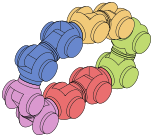
\includegraphics[width=\textwidth]{figures/ring_example.pdf}
        \caption{Loop Robot}
        \label{fig:example_roller}
    \end{subfigure}
    ~
    \begin{subfigure}[b]{0.45\textwidth}
        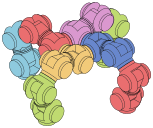
\includegraphics[width=\textwidth]{figures/spider_example.pdf}
        \caption{Walker Robot}
        \label{fig:example_spider}
    \end{subfigure}

    \caption{Examples of metamorphic systems for the case studies.}
\end{figure}

\subsection{Loop Robot}

In the first case study, I would like extend or redesign the controller
developed by \textcite{DBLP:journals/ijrr/SastraCY09}. In their work, they
designed a centralized controlled for a simple ring robot formed out of variable
number of modules (see Figure \ref{fig:example_roller} for an example of such
system). The robot can move forward by rolling. This paper leverages the
dynamics of the system to move faster compared to previous work. The controller
uses accelerometers in the modules as feedback.

I plan to introduce the following improvements:
\begin{itemize}
    \item I will transform the controller into a distributed one as the first
    step towards fault tolerance. This presents mainly a challenge in
    synchronization and information exchange.
    \item Then I would like to remove the assumption, that the individual
    modules report correct feedback. The controller should be able to deal with
    some number of units that provide incorrect feedback.
    \item If applicable, the controller should also be able to deal with some
    number of units that have faulty joints.
\end{itemize}

\subsection{Walker Robot}

In the second case study, I would like to dive deeper into the problem of
performing synchronized actions (especially movements) and more specifically,
focus on removing the bottle-neck of distributed controllers -- the bottle-neck
in form of the limited speed and bandwidth of communication lines between the
modules. There were proposed solutions for synchronization in such systems, but
they do not scale well with increased number of modules in the system.

Therefore, as a first step in this case study, I would like to take a
non-trivial configuration (e.g., walker in Figure \ref{fig:example_spider}) and
designed a mechanism for synchronous execution of a movement (prescribed by a
gait table) which scales well with the number modules. The scalability should be
achieved by dividing the system into a hierarchical cluster. Cluster members
should be able to synchronize with each other and the cluster should synchronize
among themselves. I would like to leverage findings about communication fault
tolerance from the loop robot case study and apply them to this environment as
well. Possibly, this work could be seen as extension of the concept of robotic
hormones introduced by \textcite{DBLP:conf/icra/SalemiSW01} and further extended
in \cite{DBLP:journals/trob/ShenSW02}.

The second step of this case study should be replacement of the gait tables by
individual controllers which not only require synchronization, but also require
inter-cluster feedback. I expect this part of the case study to be
generalizable.

\section{Evaluation Platform}

I would like to demonstrate the proposed solutions on a physical robots. I would
also like to make my research as reproducible as possible. That is unfortunately
quite hard in the area of robotics as one cannot easily download a robot and
test my solutions.

To achieve the best reproducibility as possible, it is crucial to use a hardware
platform which is easily obtainable. In the section \todo{Ref to existing
platforms} we provided a list of existing platforms for modular, self
reconfigurable robots. None of the platforms has manufacturing data (for
mechanical construction and PCBs) nor firmware publicly available. We also
contacted the authors if they are willing to share their design files or if
there is a possibility to buy their robots. Unfortunately none of them responded
positively. Only the authors of SMORES (\todo{citace}) responded that it would
be possible to cooperate and try our solutions on their robots at their
facility, which is not convenient.

Therefore, I set an additional goals of my PhD study: I would like to develop an
open-hardware and open-source platform for metamorphic distributed robots. This
platform should serve as tool for demonstration of my research outcomes which
allows the others to easily build their own robots and reproduce my results.
Also, by being the first open platform, it should serve as a research tool for
the others in the area.

The platform, called the RoFI platform, is part of my study I have advanced the
most so far and we introduce more in detail in Chapter \ref{chap:results}.

\section{Time Plan}

\todo{Let's make the schedule}

\chapter{Achieved Results}\label{chap:results}

This chapter sums up results achieved so far. Section \ref{platform} describes
the design of the RoFI evaluation platform and reports current progress. Section
\ref{smt} describes our experiments on solving the reconfiguration problem via
reduction to SMT.

\section{RoFI Platform}\label{platform}

We developed \emph{RoFI} -- a new platform of distributed metamorphic robots
that is open-hardware and open-source, hence almost freely available to anyone
interested. We designed our metamorphic robotic platform on top of the actual
results of other teams, and in a way, that other researchers may easily create a
physical copy of the platform on their own. We provide enough documentation to
mitigate the challenge of software development for the platform, and we
encourage others to use our platform to demonstrate the results of their work.
We believe a general publicly available platform for metamorphic robots is
beneficial for the whole community. It will prevent others from reinventing the
wheel while producing their own robots and research results.

The RoFI platform is hybrid type -- its modules are designed to fit inside
regular cubical grid. It does not define a single module shape, but it allows
the users to define custom module shapes if desired. We put several constraints
on the module shape to make the modules \emph{grid-aware} -- see Figure
\ref{fig:gridAware}. Grid-awareness allows for easier reconfiguration in dense
configurations and also combines the advantages of both, lattice type and chain
type self-reconfigurable robots. This versatility is one of the contributions of
the platform.

\begin{figure}[t]
    \centering
    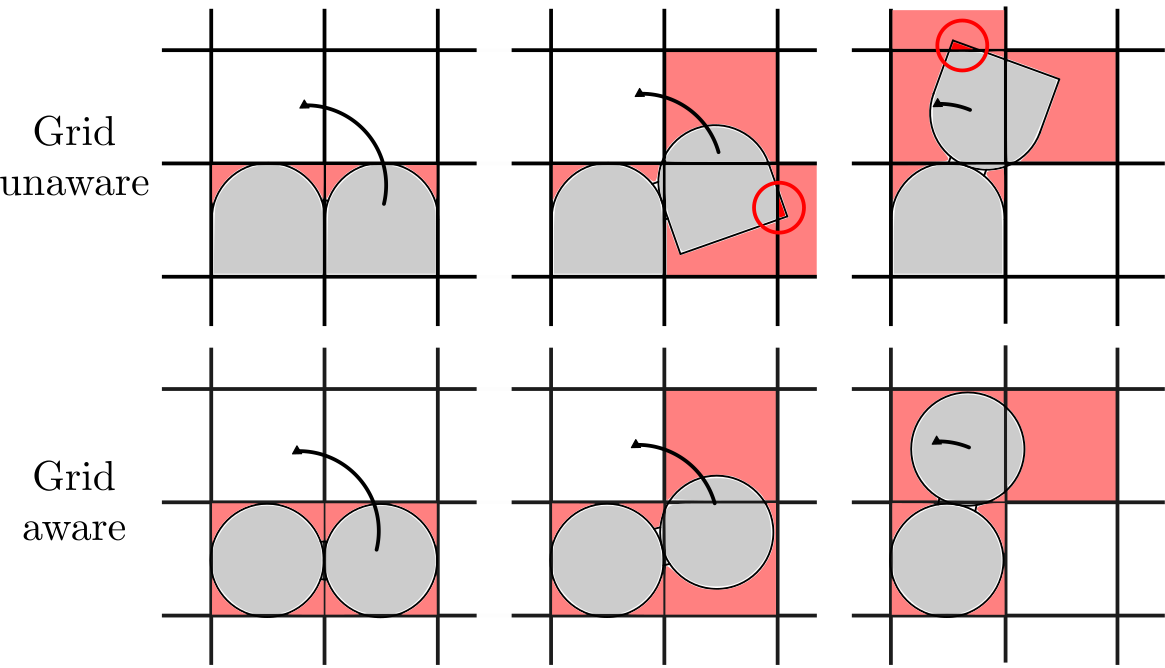
\includegraphics[width=0.7\linewidth]{figures/grid_aware.pdf}
    \caption{Illustration of grid-awareness (sequence in time). If
    a double cell module tries to move one of it bodies from right to top,
    grid-unaware module occupies extra cells of the grid.}
    \label{fig:gridAware}
\end{figure}

The grid-awareness, however, comes at the cost of increased complexity of the
connector mechanism as it need to be retractable. Therefore, we developed a
connector suitable for this task: RoFICoM \cite{DBLP:conf/iros/MrazekB19} (see
Figure \ref{fig:roficom}). RoFICoM allows for genderless grid-aware mechanical
connection between two modules with 4 symmetries. It also establishes data
communication and power sharing between the modules. It is an encapsulated
device which can be easily reused in various module types. To our knowledge, it
is the only connector which comes in the form of encapsulated device, which is
easy to integrate and is open-hardware and open-source. The connector is not
only comparable with state-of-the-art in the aspects of speed and strength, it
also outperforms it in the offered features (e.g., passive counterparts) and
miniaturization.

\begin{figure}[t]
    \centering
    \includegraphics[width=0.8\linewidth]{figures/connector_photo.jpg}
    \caption{Photo of RoFICoM.}
    \label{fig:roficom}
\end{figure}

We designed the inter-module communication such that it feeds various needs of
researchers. RoFICoMs offer point-to-point connection, which is suitable for,
e.g., digital hormone control. If broadcast, module-to-module communication or
remote control is needed we integrated RoFICoMs as another physical layer to the
popular lwIp library~\cite{lwip} implementing TCP/IP stack. Therefore, our
modules can easily interact with existing computer networks. To do so, we
designed a way for module IP address autoconfiguration and packet routing.

We demonstrate the proposed RoFI platform specification on \emph{universal
module} (see Figure \ref{fig:umPhoto}). Universal module is a 2-cell module
inspired by M-TRAN. Unlike M-TRAN it has an additional joint in the middle to
allow for more versatile reconfiguration and control (e.g., the loop
configuration can steer via this joint). The module can sense torque on all of
its axes, features an inertial measurement unit, and the connectors are capable
of time-of-light distance measuring, which serves for scanning of the
surrounding environment.

\begin{figure}[t]
    \centering
    \includegraphics[width=0.8\linewidth]{figures/um_persp.jpg}
    \caption{Photo of a single universal module.}
    \label{fig:umPhoto}
\end{figure}

Our goal is to provide means for the user to develop control software for RoFI
modules either in C++ or Python without the burden of a variety of low-level
technical issues. Therefore, we provide a set of high-level drivers and
libraries to control them. Also, we would like to allow users to easily validate
their software without the hassle of dealing with physical robots. We provide
simulation software that can directly execute the module firmware in a virtual
environment.

The whole software architecture is depicted by
Figure~\ref{fig:architecture}. The bottom layer is \emph{hardware abstraction
  layer} (HAL). HAL is a set of C++ functions, which control the basic module
capabilities directly related to the hardware, e.g., controlling joints, reading
sensors, or sending messages via connectors. All the other layers rely on HAL.

\emph{RoFI Operating System} (RoFIOS) operates on top of HAL. RoFIOS covers
essential functionality that practically all user programs rely on and is
supposed to be opaque to the user. It includes, e.g., implementation of
networking (packet routing, address mapping), module identification and
discovery, logging, firmware updates, or remote calls to the RoFIOS interface on
another module.

Directly on top of the RoFIOS runs the user firmware, which can be written
either in C++ (the preferred way) or Python. The Python programs are executed
using the MicroPython interpreter\footnote{\url{https://micropython.org/}}. User
programs do not have to be self-contained. We provide a collection of libraries
the user can use. These libraries are continuously growing and cover, e.g.,
functionality related to distributed control, environment sensing,
reconfiguration, and more.

\begin{figure}[t]
   \centering
   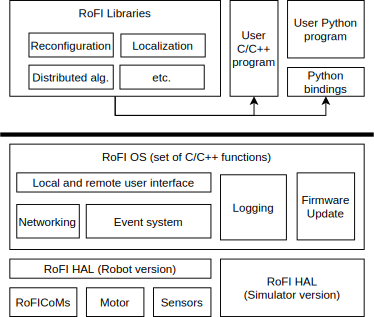
\includegraphics[width=0.7\linewidth]{figures/architecture.pdf}
   \caption{Overview of the software architecture of the RoFI platform.
   Components above other components strictly depend od them. The thick
   horizontal line defines the border between essential runtime provided by the
   modules and user programs.}
   \label{fig:architecture}
\end{figure}

Introduction of HAL allows to easily simulate programs for RoFI -- the users
just have to compile their program with simulator version of HAL. We have
developed a plugin for Gazebo~\cite{Gazebo}, which allows to simulate multiple
robots including their distributed nature -- a crash of user program does not
cause crash of the simulation. See Figure \ref{fig:gazebo}.

\begin{figure}[!t]
    \centering
    \begin{subfigure}[b]{0.45\textwidth}
        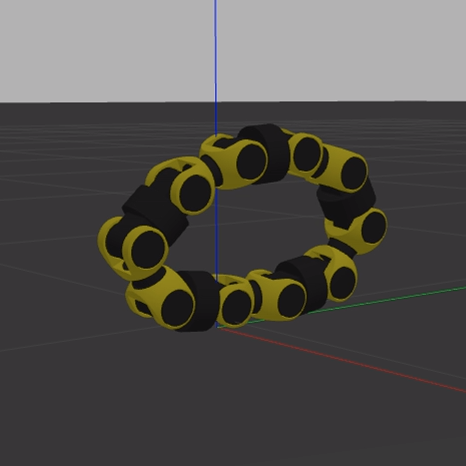
\includegraphics[width=\textwidth]{figures/sim-roller.png}
        \caption{Loop configuration}
    \end{subfigure}
    ~
    \begin{subfigure}[b]{0.45\textwidth}
        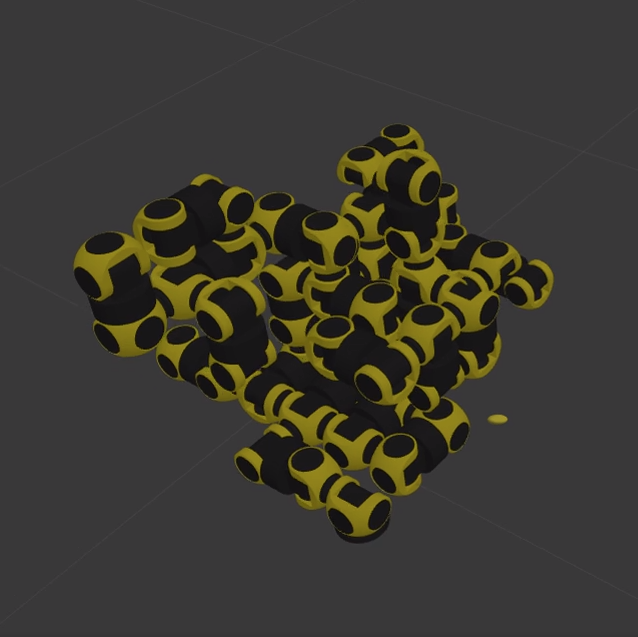
\includegraphics[width=\textwidth]{figures/sim-large.png}
        \caption{50 modules under simulation}
    \end{subfigure}

    \caption{Examples of configuration loaded into the Gazebo simulator.}\label{fig:gazebo}
\end{figure}

The RoFICoM design was already published, publication of the RoFI platform as a
whole is currently in progress. I developed the hardware and software for
RoFICoM. I am the author of the RoFI platform design -- the module shape
descriptors, I also developed the hardware and software of the universal module
of the platform. The ecosystem around RoFI was developed by students working on
the project under my guidance and assistance.

\section{Reconfiguration via Reduction to SMT}\label{smt}

One of the possible approaches to finding a reconfiguration plan is based on the
exploration of the system's state-space. This approach is without further
heuristics rather infeasible as the state-space of all possible transformations
is vast. The state-space exploration is a widely used technique also in the
field of formal verification. In this field, recently, many tools stopped
directly exploring the state-space of a system, and instead, they are reducing
the problem to the problem of \emph{satisfiability modulo theory}
(SMT)~\cite{DBLP:series/faia/2009-185}. In a nutshell, the verification tool
constructs a logic formula such that it is satisfiable if and only if the
erroneous state of the system under inspection is reachable. After that, the
formula is passed to an SMT solver, which decides its satisfiability. The
SMT-reduction based approach has proven to be quite effective in the
verification community as it leverages the sophisticated heuristics implemented
in the solvers.

In this work, we explore the possibility of applying a similar approach -- we
want to leverage SMT and SMT solvers to tackle the problem of reconfiguration.
Our basic goals are twofold, first, to find out whether the suggested way is a
viable one in terms of practical usability, and second, to see how much of a
performance boost we can expect in the future from the continuous development of
SMT solvers. Compared to work by \textcite{DBLP:journals/pcs/GorbenkoP12}, our
approach yields collision-free reconfiguration plans.

The \emph{reconfiguration plan} for two configurations $c_{initial}$ and
$c_{target}$ is a sequence $(c_{initial}, c_2, \cdots, c_{n - 1}, c_{target})$
of configurations such that all configurations are strongly connected (as we
model modules without locomotion) and also for each two consecutive
configurations $c_i$ and $c_{i+1}$ it holds that either they are the same or
$c_{i+1}$ can be obtained from ${c_i}$  by applying exactly one of the following
actions: releasing some connections, establishment of new connections, or
joints' movement.

Let us assume for now that we can construct a first-order formula
$\pi_{n}(c_{initial}, c_{target})$ in the theory of non-linear real arithmetic
such that the $\pi_n$ is satisfiable if and only if there exists a valid
reconfiguration plan of length $n$ from $c_{initial}$ to $c_{target}$. Then we
can pass $\pi_n$ to an appropriate solver and find out whether it is satisfiable
or not. If so, we can easily extract the reconfiguration plan from the model of
the formula.

To find the shortest path, we may iteratively construct $\pi_2$,
$\pi_3$, $\pi_4$, $\cdots$ to find out the first satisfiable formula. The
possible improvement of this naive approach would be to guess an upper bound on the
length of the shortest reconfiguration plan and use binary search to find the
lowest $n$ for which $\pi_n$ is satisfiable.

The challenge of this approach lies in the construction of $\pi_n$. In our work,
we tested several approaches for expressing the formula. We tackle it by
introducing a concept of \emph{external} and \emph{internal} representation of a
configuration. The internal provides a trivial way to  encode a transition from
one configuration to another, the external provides a trivial ways encoding
configuration validity. Therefore, we only need to express a relation between
these two representations in a the logic. The naive expression does not work as
the formula is large and state-of-the-art solvers struggle with trigonometry. We
solve this problem using quaternions to express modules' orientation. We also
propose a suitable discretisation to circumvent the need to use an universal
quantifier as the solvers do not handle universal quantification.

We evaluated our work on several version of the following solvers Z3
\cite{DBLP:conf/tacas/MouraB08}, SMTRAT \cite{DBLP:conf/sat/CorziliusKJSA15},
dReal \cite{DBLP:conf/cade/GaoKC13}, Yices2 \cite{DBLP:conf/cav/Dutertre14},
CVC4 \cite{DBLP:conf/cav/BarrettCDHJKRT11}. Based on our experimental
evaluation, our approach is comparable to the existing state-of-the-art in this
area and therefore, is currently unapplicable in practice. However, during the
evaluation of historical version of the solvers we noticed performance
improvements between the versions, thus this approach might be viable in the
future.

Publication of this work is currently in progress. I am a co-author
of the core idea, I am the author of the quaternion-based optimization. I also
created a reference implementation and I performed the experiments.

\section{Publications}

\begin{itemize}

    \item \fullcite{DBLP:conf/iros/MrazekB19}

    I am the main author of the design and paper text.
\end{itemize}


\chapter*{Bibliography}
\addcontentsline{toc}{chapter}{Bibliography}
\markboth{}{} % avoid headers from last chapter in bibliography
\printbibliography[heading=none]

\appendix


\end{document}
